\section{Introduction}


Since the publication of RT-1 \cite{RT-1} the robotics research is undergoing a prolific period focused around foundation models. The central promise of this paradigm is the development of generalist policies that aim to achieve general-purpose embodied intelligence, capable of complex interactions within unstructured environments. This shift mirrors advancements in Machine Learning, particularly in Natural Language Processing and Computer Vision, where large pretrained models have demonstrated remarkable success.

\begin{wrapfigure}{r}{0.45\textwidth}
    \centering
    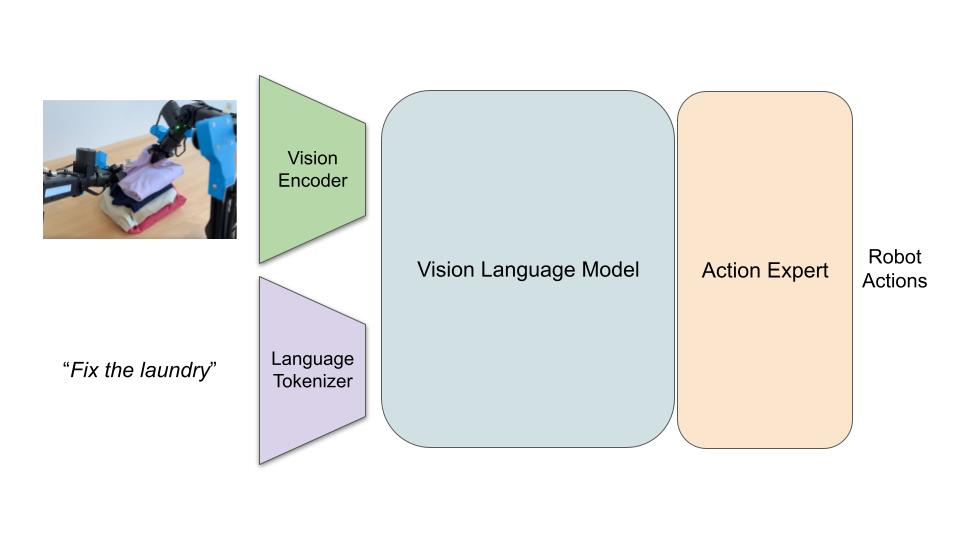
\includegraphics[width=0.45\textwidth]{images/vla.jpg}
    \caption{VLA abstraction}
    \label{fig:vla_abstraction}
    % https://docs.google.com/presentation/d/1F3-KIjQxwBtXfJAlc9_vwuBLSGuZqcXqZ7_GfxX5kYY/edit?usp=sharing
\end{wrapfigure}

Robotics foundational models, often referred to as Vision-Language-Action (VLA) models, is the name of the policies emerging from this paradigm shift (Figure \ref{fig:vla_abstraction}). This nomenclature reflects their modality inputs, vision and language, and outputs, action. Leveraging techniques such as Imitation Learning, Reinforcement Learning, and Self-Supervised Learning, these models have demonstrated remarkable capabilities in dexterous manipulation across multiple tasks, offering a degree of generalization over robot embodiments and environments. A key enabler of this progress is the rise of large-scale pre-training which utilize vast datasets to construct general-purpose representations, applicable across diverse robotic settings, tasks, and embodiments \cite{TransferWelle}.


\section{Goals and Objectives}
Due to their rapid success, the field lacks a standardized benchmarking literature, a critical component for ensuring coherent and equitable expansion. While some work, such as the $\pi_0$ model \cite{pi_zero}, showcase tasks involving deformable object manipulation (e.g., laundry folding), a unified approach for comparing models remains absent. Current efforts often focus on testing single models rather than comparing multiple foundational models to elucidate their differences. This proposal aims to address this gap by developing a Deformable Object Manipulation Benchmarking suite for Robotics Foundation Models, fostering a deeper understanding of their capabilities and limitations. Specifically, we will empirically evaluate how the choices made when building a model (architectural, training recipe, tasks covered, etc.) affect performance on the model capabilities.

% For example a key architectural feature, the Action Decoder, has been implemented in different ways, diffusion transformer \cite{Gr00tN1} or flow matching \cite{pi_zero} or direct decoding from the VLA \cite{OpenVLA}, and a comparative study will help understand the impact of this choice.

\subsection{Overall Goal}<

This project aims to deliver:

    \begin{enumerate}
        \item Benchmark suite to evaluate robotics foundational models against deformable object manipulation
        \item Evaluation protocol, applied to the selected policies 
        \item Summarization of the work in a paper
    \end{enumerate}


\subsection{Specific Objectives:}
    \textbf{Literature Review}
        Conduct a comprehensive review, including but not limited to:
        \begin{itemize}
            \item Existing robotics benchmarks, evaluation methodologies, and taxonomies focusing on deformable object manipulation.
            \item Robotics foundational models, emphasizing architectures, training data, and intended capabilities.
        \end{itemize}
    \textbf{Benchmark Design}
        Propose a standardized benchmark suite that integrates and/or extends existing ones and an evaluation protocol. This includes defining clear metrics to provide multidimensional insights of the models' abilities beyond mere performance, such as:
        \begin{itemize}
            \item \textit{Generalization}: Formalize the variations across environments (ex: 1. RPL Laboratory 2. Simulation (GarmentLab, DaXBench, ...), tasks (ex: Cloth Folding, Rope knotting, Sponge ..., Liquid Pouring), and robot embodiments (..., SO-100). (FORMALIZE BETTER?)
            \item \textit{Data efficiency}: Specify how to measure performance across scaling the number of samples the policy consumes: zero-shot, few-shot performance. (FORMALIZE BETTER?)
            \item (Stretch Goal) \textit{Context horizon}: Expand the type of tasks taken into account to quantitatively investigate the horizon each model is able to sustain to solve a task: short-term versus long-term task performance. (FORMALIZE BETTER?)
            \item (Stretch Goal) \textit{Explainable AI}: usage of explainable AI methods such as probing \cite{Probing-VLA} to gain measures of understanding from the internal feature representations of the model. (FORMALIZE BETTER?)
        \end{itemize}
        % \item \textbf{Validation Strategy:} Outline a strategy for validating the proposed benchmark's relevance and effectiveness, potentially including correlating benchmark results with real-world robot performance or through expert evaluations to ensure the benchmark captures ``sense of reality'' (i.e., reflects real-world applicability).

    \textbf{Evaluation}
        Implement the defined evaluation protocol and apply it to a selected set of publicly available foundation models, following the benchmark's recipe. A candidate list of the foundational models to test is:
        \begin{itemize}
            \item $\pi_0$, \cite{pi_zero}
            \item OpenVLA, \cite{OpenVLA}
            \item (Stretch Goal) Gr00t \cite{Gr00tN1}
            \item (Stretch Goal) Octo \cite{Octo}
        \end{itemize}
        


\textbf{Significance:} This work addresses the current lack of standardized benchmarking for robotics foundation models, particularly for the challenging deformable object manipulation tasks. By providing a common evaluation framework, this benchmark aims at facilitating comparisons and guide future research towards the development of more capable robotic systems.